\documentclass[english]{DESCARWINreport}

\usepackage{times}
\usepackage{helvet}
\usepackage{courier}
\usepackage{graphicx}
\usepackage{multirow}
%\usepackage[utf8]{inputenc}
\usepackage{algorithm}
\usepackage[noend]{algorithmic}
\usepackage{amsmath}
\usepackage{amsfonts}
\usepackage{amssymb}
\usepackage{array}
\usepackage{caption,subfig}
% \usepackage{subfigure}
\usepackage{lscape}

%%%%%%%%%%%%%%%%%5 includepdf
\usepackage[final]{pdfpages}

\algsetup{indent=1.8em}
\renewcommand{\algorithmiccomment}[1]{// #1}
\newcommand{\pp}{planning tasks}
\newcommand{\PP}{planning task}
\newcommand{\dae}{{\em Divide-and-Evolve}}
\newcommand{\DAEI}{{\sc D\&E}}
\newcommand{\DAEII}{{\sc DaE2}}
\newcommand{\DAE}{{\sc DaE}}
\newcommand{\DAEX}{{\sc DaE$_{\text{X}}$}}
\newcommand{\DAEYAHSP}{{\sc DaE$_{\text{YAHSP}}$}}
\newcommand{\CPT}{{\sc CPT}}
\newcommand{\LPG}{{\sc LPG}}
\newcommand{\LAMA}{{\sc LAMA}}
\newcommand{\TFD}{{\sc TFD}}
\newcommand{\YAHSP}{{\sc YAHSP}}
\newcommand{\LAO}{{\sc LaO}}
\def\MODAE{{\sc MO-DaE}}
\def\ZENO{{\sc Zeno}}
\def\MULTIZENO{{\sc MultiZeno}}
\def\PARAMILS{{\sc ParamILS}}

\def\UU{{\mathbb{U}}}

%\title{DESCARWIN\\\bigskip {\em \LARGE The Marriage of Descartes and Darwin}\\\bigskip \bigskip \bigskip \bigskip \bigskip \bigskip \bigskip {\LARGE WP1: the \DAEX\ Planning System}}
\title{DESCARWIN\\\bigskip {\em \LARGE The Marriage of Descartes and Darwin}\\\vspace{8cm} 
{\LARGE D2.3\\
Experiments on On-Line Parameter Control}}
\date{\today}
\laboratory{TRT - INRIA - ONERA}
\docref{62 441 217-179-1}

\revision{-}

\setlength{\parindent}{0cm}
\setlength{\parskip}{2ex plus 0.5ex minus 0.2ex}

\newcounter{hyp}
\setcounter{hyp}{1}
\newcommand{\hyp}{H\thehyp\stepcounter{hyp}}
\newcounter{defi}
\setcounter{defi}{1}
\newcommand{\defi}{D\thedefi\stepcounter{defi}}
\newcounter{con}
\setcounter{con}{1}
\newcommand{\con}{C\thecon\stepcounter{con}}

% Pour r�duire globalement l'espace entre les items d'une liste
% on peut �galement utiliser le bout de code suivant de M. Wooding
% Les param�tres utilis�s pour d�finir cette mise en page
% sont les suivants :
% \topsep espace vertical suppl�mentaire (ajoute � \parskip)
% 	ins�r� entre le texte pr�c�dant la liste et le 1er objet
% 	de la liste
% \partosep espace vertical suppl�mentaire ins�r� devant la liste
% 	si celle-ci est pr�c�d�e d'une ligne blanche
% \itemsep espace vertical suppl�mentaire (ajout� � \parsep)
% 	ins�r� entre les �l�ments d'une liste.

%%%% debut macro %%%%
% \makeatletter
% \toks@\expandafter{\@listI}
% \edef\@listI{\the\toks@\setlength{\parsep}{0pt}}
% \edef\@listI{\the\toks@\setlength{\topsep}{0pt}}
% \makeatother
%%%% fin macro %%%%


\begin{document}

\maketitle

%\cleardoublepage

\begin{revisions}
\begin{revtable}
\dates{APR. 13, 2011}{}{}{}
\writers{Matthias Brendel\\Johann Dr\'eo\\Mostepha Khouadjia\\Pierre Sav�ant\\Marc Schoenauer\\Vincent Vidal}{}{}{}
\approvers{P. Sav\'eant}{}{}{}
\end{revtable}
\begin{revisionlabels}
\revlabel{initial version}
\revlabel{}
\end{revisionlabels}
\end{revisions}

\begin{abstract}
This deliverable does not exactly match its initial description that had been made in the original Description of Work of the DESCARWIN proposal. It turned out indeed that the methods that we had in mind when writing the proposal couldn't work in the framework of AI planning as approached with \DAE, due to the very small number of different fitness values encountered during \DAE\ runs. This will be detailed in the first Chapter 2 of this deliverable. \\

Nevertheless, the Learn-and-Optimize framework (as described in Deliverable 2.2, Chapter 2) can be thought of as an intermediate method between off-line and on-line learning: if the optimizer is installed in some production line, and has to solve a sequence of instances of the same domain, then the instance-based method Learn-and-Optimize is a way to adjust the parameters of the optimizer to the current instance automatically, without any human intervention, i.e., at runtime. A lot of efforts were devoted to further developments of the \LAO\ method \ldots that turned out however to fail to improve the initial results. Furthermore, this was confirmed when \LAO\ was submitted to the IPC-2011 competition, where unfortunately it obtained rather poor results - in part only because of the lack of time for preparation before the post-doc in charge, M�ty�s Brendel, left the project. This is detailed in Chapter 3, and a copy of the paper that was submitted with the candidate planner for the competition is appended.\\

Also, and as planned in the original workplan, our effort had to turn to the multi-objectivization of Divide-and-Evolve, and of course this also includes adapting the parameter tuning methodology to the multi-objective context. It also turned out that a new framework for off-line parameter tuning, called ParamILS (see reference [4] in Chapter 4), developed at University of British Columbia, was gaining popularity, because of the excellent ratio (performance / CPU cost) it obtained compared to the Racing procedure that we had been using up to then (described in Chapter 1 of Deliverable 2.1). We hence decided to modify our off-line tuning method and to exclusively use ParamILS further on. Details of ParamILS and our implementation are briefly given in Chapter 4, together with some samples trajectories in the fitness space.\\

As mentioned above, the new framework was initially set up for the multi-objective work on \DAE, and one issue that had not been planned ahead arose: which metric use within ParamILS to assess the performance of the different parameter sets? For the Pareto-based multi-objective algorithms, the {\it hypervolume} was an obvious candidate, and it turned out it performed very well indeed. But for the aggregation approach, in which a single-objective \DAE\ is used to optimize a weighted sum of the objectives, the obvious choice was to use, for each of the runs optimizing a weighed sum of objectives, the very same fitness, i.e., the very same weighted sum. However, it turned out that a better choice was to also use the {\it hypervolume} indicator, even though different from the metric that each run optimizes, as demonstrated in Chapter 5. 

This work was published as ``Khouadjia, M.R. , Schoenauer, M. , Vidal, V. , Dr�o, J. and Sav�ant, P.. Quality Measures of Parameter Tuning for Aggregated Multi-Objective Temporal Planning. In Panos Pardalos and Giuseppe Nicosia, eds.: LION'7 -- 7th Learning and Intelligent OptimizatioN Conference, Springer Verlag, LNCS. Catania, Italy. January 2013.''

A copy of the published paper is included after a brief recall of the context and main results, in Chapter 5.

\end{abstract}

\tableofcontents

% \newpage
% 
% \chapter{Introduction}

\newpage
\chapter{Failure of on-line control methods based on operator rewards}

When the DESCARWIN proposal was written, we had a clear idea in mind regarding on-line parameter control (see Deliverable 2.1 for the list of the now-standard vocabulary): because the INRIA partner had been involved in several works regarding on-line parameter control, we anticipated that the same approaches could be used within \DAE\ framework. In particular, this concerned the on-line parameter control, where the parameters are modified during the run, depending on the history of the search, the idea was to port Adaptive Operator Selection (AOS) methods, for which the INRIA partner had a large expertise (PhD thesis of Alvaro Fialho entitled {\em Adaptive Operator Selection for Optimization} and defended in December 2010).

The basic idea of AOS methods (see Deliverable 2.1, Chapter 4) relies on two components: whenever an operator is applied, its impact is recorded, and some {\em reward} is given to the operator, usually based on the fitness improvement, i.e., depending whether the fitness of the offspring is better than that of the parent(s). The second component is a decision mechanism that uses the past rewards of all operators to decide which one to use next. There are several such decision mechanisms, e.g. Probability Matching, Adaptive Pursuit, and the family of Multi-Armed bandit based methods developed by Alvaro Fialho in his PhD. But all of them are based on some reward that is computed from the fitness improvement brought by the operators - and such rewards are zero if the fitness does not increase in the population. Note that this is true even for the rank-based mechanism that is described in detail in Chapter 4 of Deliverable 2.1, rank-based mechanism that was our preferred candidate AOS for \DAE\ because of its invariance by monotonous transformation of the fitness, and is hence independent of any fitness scaling, the Achille's heel of most AOS method based on fitness improvement.

\begin{figure}[h!]
\begin{center}
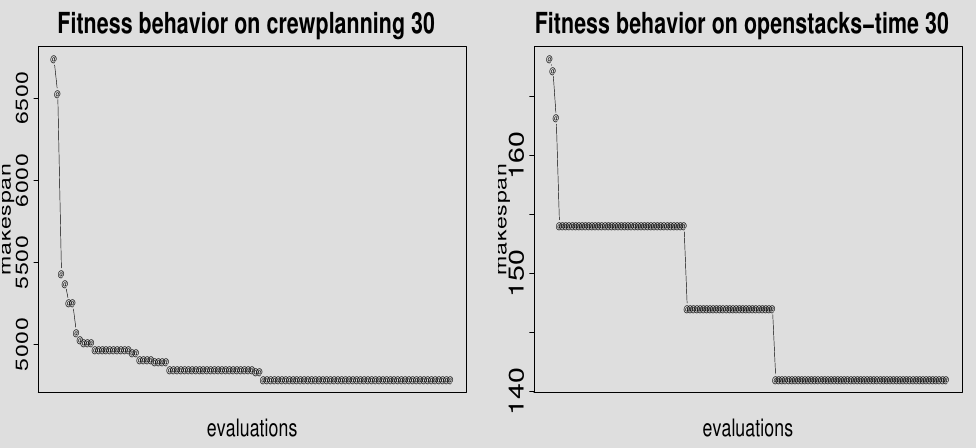
\includegraphics[width=0.9\textwidth,height=6cm]{fitnessBehavior.png}
\end{center}
\caption{Typical evolution of the fitness during some \DAE\ runs.}
\label{fig:fitnessImprovement}
\end{figure}


During \DAE\ runs, however, it turned out that very few fitness improvements do take place -- mostly because there are very few possible fitness values, at least when reaching regions of the search space around the optimum. Figure \ref{fig:fitnessImprovement} displays typical evolution of the best fitness in the population during two \DAE\ runs, for two large instances of two different IPC domains, {\tt crewplanning} and the temporal {\tt openstacks}: the best fitness in the population goes through only 3 values for {\tt openstacks}, and less than a dozen for {\tt crewplanning}. There is hence little hope that AOS based on fitness improvement (even, as said above, the champion rank-based AOS) can learn which operators perform best with so few example of improving operations.

After some preliminary experiments that confirmed this trend, it was decided to 
\begin{enumerate}
 \item not waste any more time trying to run some Adaptive Operator Selection method to \DAE\ context
 \item investigate the {\em Learn-and-Optimize} (\LAO) approach that had been developed with M�ty�s Brendel within the project; Indeed, \LAO\ can be seen as a somehow intermediate method between off-line and on-line method, as it learns how to predict the best parameters from solved instances (hence off-line), but later determines the optimal parameters for new and unseen instances: this is done automatically, if not during the run -- and at least a single run is needed for each new instance, by contrast to pure off-line method who require many runs to adjust the parameters for any instance.
 \item put more efforts on the multi-objective case, because the topic was gaining interest in the AI Planning community (again -- see Deliverable 3.3). And it turned out that indeed some more efforts were needed for off-line parameter setting when going from single- to multi-objective contexts.
\end{enumerate}
The rest of the deliverable will thus detail the work done on \LAO\ following the preliminary work that has been introduced in Deliverable 2.2, Chapter 3, that unfortunately didn't bring much improvement over the preliminary results. Then we will turn to the specific work done in the context of Pareto-based multi-objective optimization, in relationship with Deliverable 3.3.

\newpage	
\chapter{Progress on LaO}
\section{New results: ICAPS-2011 and IPC-2011}

A first research line was to continue the work on \LAO\ that had been started in early 2011, and was published at GECCO as a poster, and in the selected papers of the Evolution Artificielle conference (Hao et al., eds, LNCS 7401, Springer Verlag, pp 159-170, 2012). These results have been described in Deliverable 2.2, where Chapter 3 contains the seminal paper on \LAO\ that was reduced to a 2 pages poster description at GECCO, and slightly reduced for space constraint reasons in the LNCS volume of Evolution Artificielle.

These results were detailed and slightly extended in a paper presented at the {\em Planning and Learning Workshop} at ICAPS-2011, that is included later in this Section. The conclusions remain the same: some marginal improvement over the default parameter set could be obtained using \LAO\ with only a few iterations. However, the inter-domain generalization capabilities remain unknown -- or, more precisely, though not reported in the paper, the first attempts proved to give poor results, even with more iterations. The main critical issue probably still was the quality of the feature set, that was far too limited to actually take into account the characteristics of the instances that could lead to the optimal parameter set, undermining the critical hypothesis of the algorithm.

In the meantime, \LAO\ also entered the IPC-2011 competition (that took place at ICAPS-2011), in the Learning Track. Unfortunately, it ranked only 7th out of 9 candidates, being unable to solve several of the hidden instances in spite of the learning phase. This is attributed to the poor generalization capacities of the framework.

\newpage
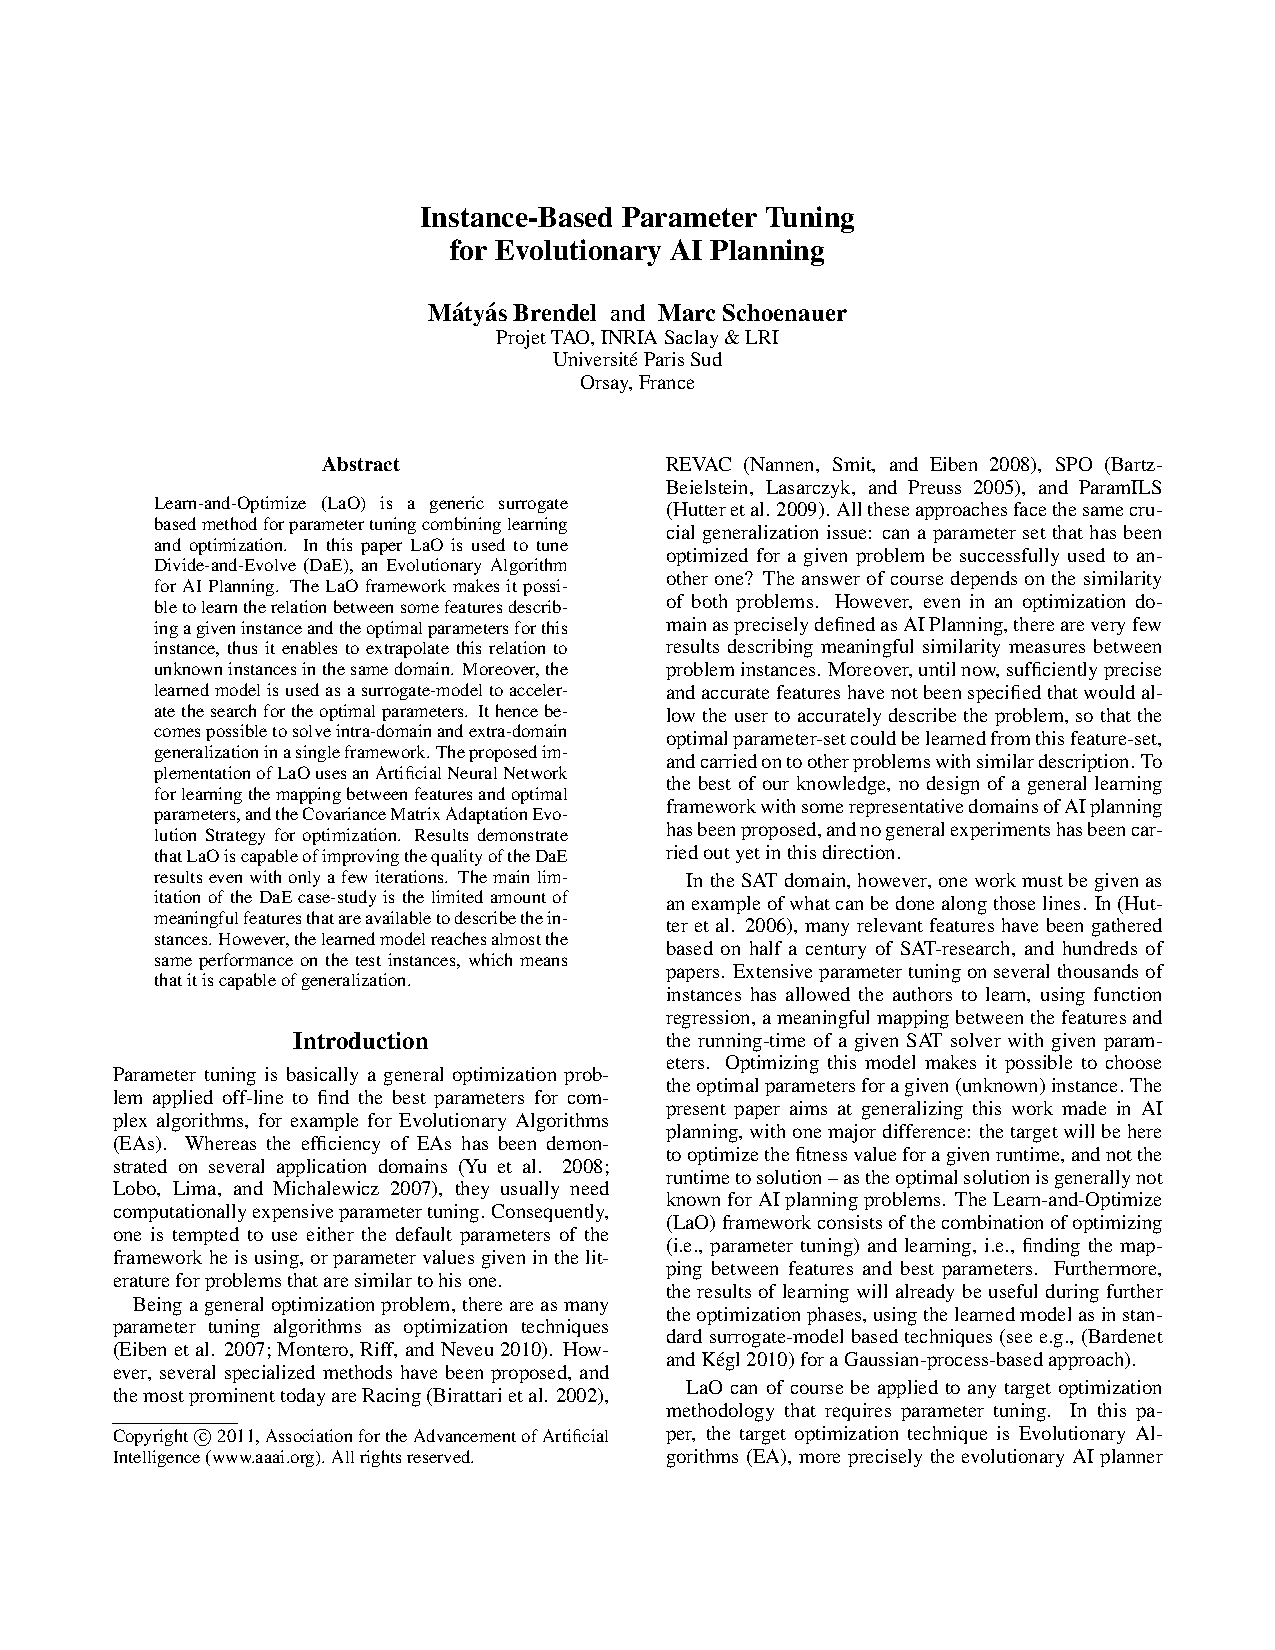
\includepdf[height=30cm,pages=-,offset=2.2cm -4cm]{icaps2011.pdf}
\newpage

\section{Further Work on LaO}
Several research directions have been explored from there on to try to improve the results of the \LAO\ framework. But none of them was able to provide significant improvements on the AI Planning domains. As a consequence, none has lead to any publication -- as unfortunately nowadays in science, negative results are no results to publish.

The first direction regards the {\bf features} are used to characterize the different instances. In the published results, the same initial 12 features have been introduced and used. But we suspect that these original 12 features are not sufficient to capture the peculiarities of the instances w.r.t. the parameters of the planner. Indeed, adding new features is a way to increase the chances to be able to identify relevant characteristics, and derive an accurate model to predict some good values for the parameters; however, the more features the higher the chances to hinder the learning phase with useless information, eventually hiding the correct correlation and resulting in worse results.
Note that, even though they didn't improve the results, these features are in the code delivered as D2.4.

Two sets of possible interesting features have been explored.

\begin{itemize}
\item Beyond the 12 initial features, we developed statistical features of the "histogram type``, e.g., the chronopartition, number of types and number of terms. All these features result in a histogram, i.e. a series of numbers, which can be interpreted as a distribution. For each of these, we computed the mean, the median, and the value at the first and third quartile. Using them either alone or in addition to the initial 12 features did not improve the results with independent tests. 

\item Furthermore, we also developed the probing features, i.e., running a naive heuristic (e.g., greedy, depth first, \ldots) for a short time and recording the improvements. Using such features, again, did not improve the results. None of these features harmed a lot, but one could nevertheless see some degradation of the results -- which is why this line of research was abandoned. In spite of the fact tests with the additional features 24 or 32 features were made on around 100 instances, we thought that there was no risk of over-fitting. However, it seems there was a slight over-training, as the results on the test set were worse,whereas the results on the training set were slightly improved. But the main problem was of course that these new features were not useful at all.
\end{itemize}

% Some other investigations regarded the use of another model for the learner. We tried to use Rank-SVM regression, in order to avoid possible scaling issues with the fitnesses. Again, 
% 
% 
% XXXXXXXXXXXXXXXXX
%  We developed the indirect model with Artificial Neural Networks. The indirect model was optimized using CMA-ES algorithm when it was queried for new parameters. However, this approach resulted in a decrease of around 0.8 in ratio compared to the default parameters.
% 
% Also we tried an indirect model using Rank-SVM regression. Here, after optimizing only in a small neighborhood around the default parameters, the decrease (a ratio with defaults parameters) was slightly bellow 1. So, the indirect models did not really work out.

Another quite worrying issue is that of generalization: a model trained for one domain was never good enough for another domain, as several experiments with different domains and different sets of instance demonstrated. We also tried to train a big, domain-independent model using all instances of the IPC-2008 domains, meaning that we were using more than 500 instances for training. This did not work either when tested on an independent test set, and again the ratio of performance when compared to the default parameter set was around 0.8 (performance decrease). So learning a model more general than one domain seems to be a very hard task for \LAO. 


\section{Conclusion on LaO}
At the light of the results presented in Deliverable 2.2 and above, and considering the fruitless efforts that have been deployed to overcome the difficulties in improving the initial results and obtain competitive results with other approaches, the \LAO\ path seemed rather narrow and steep.

Furthermore, an additional argument was that the multi-objectivization of \DAE\ had been delayed far too long, and was becoming urgent as other researchers started to investigate multi-objective problems in AI Planning.

Hence, it was decided for this WorkPackage, from this point, on to abandon all research on \LAO\ and to concentrate on the multi-objective \DAE.

\newpage

\chapter{ParamILS: A robust and efficient framework for off-line tuning}

It is widely acknowledged today that off-line parameter tuning has somehow reached a mature state, and is considered a mandatory step when evaluating and validating the performance of any optimization or machine learning algorithm. This recent trend, advocated by Holger Hoos (University of British Columbia) under the name of {\em Programming by Optimization} (see e.g., http://www.prog-by-opt.net/ and references herein) has however been started many years ago in the Evolutionary Computation community, with the seminal work {\em  Parameter control in evolutionary algorithms} by A.E. Eiben, R. Hinterding, and Z. Michalewicz in 1999 \cite{eiben99parameter}, and the many different (meta-)algorithms that have been proposed in that respect (see Deliverable 2.1, Section 3.3.2 for detailed descriptions). However, the situation seems to have slightly evolved since that Deliverable was written, and whereas all our past experiments were using some Racing procedure, the ParamILS framework developed at University of British Columbia was found better performing, and more flexible and general purpose tool than all EC-specific approaches (like SPO \cite{SPO:CEC05} and REVAC \cite{NannenE07} for instance), and than the F-Race \cite{birattari2002} framework proposed by IRIDIA. \\

The off-line parameter tuning problem can be informally stated as a meta-optimization algorithm: given an algorithm, a set of parameters for the algorithm and a set of input data, 
find parameter values under which the algorithm achieves the best possible performance on the input data.
To avoid potential confusion between algorithms whose performance is optimized and algorithms used for carrying out that optimization task, we refer to the former as target algorithms and to the latter as configuration procedures (or simply configurators). This setup is illustrated in Figure~\ref{fig:paramIlsframework}.

\begin{figure}[h!]
 \centering
 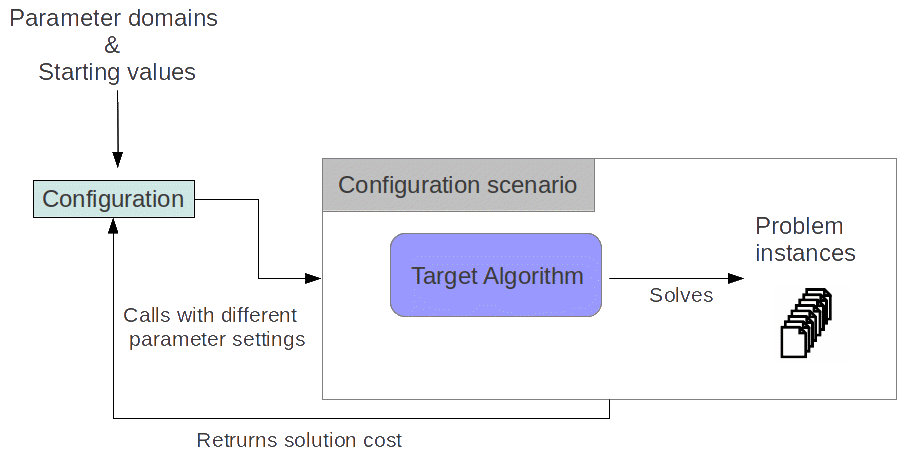
\includegraphics[width=0.8\textwidth]{schemaParamILS.png}
 \caption{ParamILS framework: A configuration scenario includes an algorithm to be configured and a collection of problem instances.
A configuration procedure executes the target algorithm with specified parameter settings on some or all of the instances, receives information about the performance of these runs, and uses
this information to decide which subsequent parameter configurations to evaluate.}
\label{fig:paramIlsframework}
\end{figure}

ParamILS~\cite{hutter2009paramils} is suited to any parameterized algorithm whose parameters can be discretized. ParamILS searches through the space of possible parameter configurations, evaluating configurations by running the algorithm to be optimized on a set of benchmark instances. Users should provide
\begin{itemize}
\item a parametric algorithm A (executable to be called from the command line),
\item  all parameters and their possible values (parameters need to be configurable from the command line),
\item all parameters and their possible values (parameters need to be configurable from the command line),
\item and a set of benchmark problems, S.
 \end{itemize}

The idea behind ParamILS is to use iterated local search (ILS) \cite{lourencco2003iterated} to search for performance-optimizing parameter configurations. ILS is a prominent stochastic
local search method that builds a chain of local optima by iterating through a main loop consisting of (1) a solution perturbation to escape from local optima, (2) a subsidiary local search procedure and (3) an acceptance criterion to decide whether to keep or reject a newly obtained candidate solution.

Users can choose from a multitude of optimization objectives, reaching from minimizing average runtime to maximizing median approximation qualities. ParamILS then executes algorithm A with different combinations of parameters on instances sampled from S, searching for the configuration that yields overall best performance across the benchmark problems. The issue of which instances to consider (how to sample S) will not be discussed here, even though it is of utter importance, as demonstrated in the single-objective case with the {\it racing} procedure in this project (see Deliverable 2.2, Chapter 3).

Another point of view on ParamILS is that of a manually-executed local search with restarts in parameter configuration space. More precisely, it is an iterative first improvement procedure with restarts, with a search space consisting of all possible parameter configurations, an objective function that quantifies the performance achieved by the target algorithm with a given configuration, and a neighborhood relationships based on changes on one single parameter value at a time. 

When dealing with multi-objective problem, the optimal solution of the target algorithm is a set of non-dominated solutions as close as possible from the true Pareto set, i.e., the optimal trade-offs between the different conflicting objectives. In order to measure the quality of the output $A$ of the target algorithm, we need some reference set $Z^*_N$, and compute the hypervolume difference between $A$ and $Z^*_N$ \cite{Zitzler2004}. The smaller this (positive) measure, the better the approximation of $Z^*_N$ by $A$. 
Whenever available, the reference set $Z^*_N$ is chosen as the true Pareto set. However, and in particular in real world problems, the true Pareto set is not known, and the reference set is chosen as non-dominated points from the union of all approximations ever obtained.

Figure \ref{fig:paramILS-trajectories} displays the behavior of ParamILS when optimizing the parameters of the four candidate multi-objective schemes for \MODAE\ that are compared in Deliverable 3.3, Chapter 2. The different restarts are clearly visible (sudden increase of the hypervolume). Furthermore, ParamILS very often discovers the best setting rather early in the run, but keeps on trying new configurations, somehow validating the default values that are used as a starting point. However, it also happens (not on these plots) that the best configuration is found later in the run. 


\bibliographystyle{plain}
\bibliography{ppsnb}

\newpage
\begin{figure}[h!]
 \centering
 \subfloat[zeno3$-{cost}$]{ 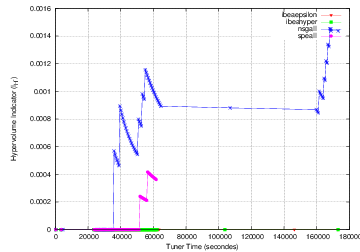
\includegraphics[width=0.45\textwidth]{zeno3e_Add_paramils.png}}
  \subfloat[zeno3$-{risk}$]{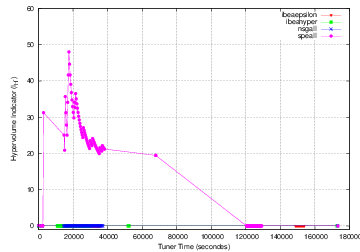
\includegraphics[width=0.45\textwidth]{zeno3e_Max_paramils.png}}\\
  \subfloat[zeno6$-{cost}$]{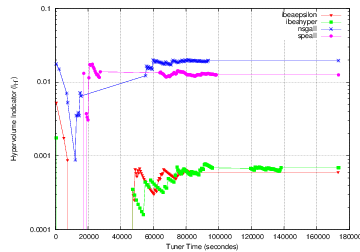
\includegraphics[width=0.45\textwidth]{zeno6e_Add_paramils.png}}
  \subfloat[zeno6$-{risk}$]{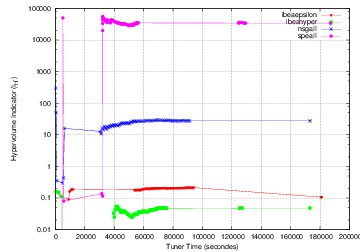
\includegraphics[width=0.45\textwidth]{zeno6e_Max_paramils.png}}\\
  \subfloat[zeno9$-{cost}$]{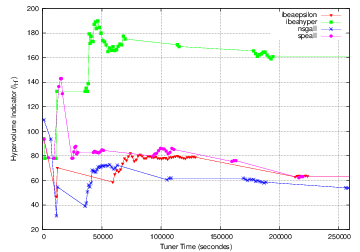
\includegraphics[width=0.45\textwidth]{zeno9e_Add_paramils.png}}
  \subfloat[zeno9$-{risk}$]{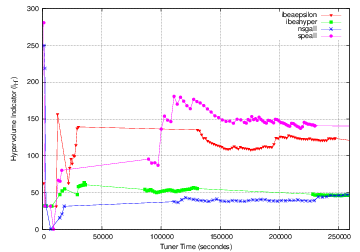
\includegraphics[width=0.45\textwidth]{zeno9e_Max_paramils.png}}\\
\caption{Sample ParamILS trajectories for the different algorihtms that are compared in the EMO 2013 paper (see Deliverable 3.3 Chapter 2).}
\label{fig:paramILS-trajectories}
\end{figure}


\newpage
\chapter{Using ParamILS for multi-objective parameter setting: the case of the aggregation approach}

As discussed in the previous chapter, when tuning the parameters of some target multi-objective algorithm (evolutionary or not), a natural metric for measuring the performance of the algorithm is the hypervolume w.r.t. some reference set (if at all possible, the true Pareto front of the problem at hand). This metric has been used in all experiments done in this project for Pareto-based multi-objective optimization (see Deliverable 3.3 Chapter 2).

On the other hand, when tackling some single objective optimization problem and aiming at solution quality, the usual metric used for ParamILS is the best fitness reached by the target algorithm for a given parameter set. 

Furthermore, the validation of the Pareto-based multi-objective approach needs to achieve some comparison with the classical and straightforward aggregation approach (see Deliverable 3.3 Chapter 3), in which you run several single-objective runs trying to optimize a weighted sum of the objectives, say $\alpha F_1 + (1-\alpha) F_2$, $F_1$ and $F_2$ being the two objectives, and $\alpha$ taking values in $[0, 1]$ (such a run is called $\alpha$-run). Hence, in order to give the best chances to the aggregation approach, we decided to tune independently the parameters for each of the $\alpha$-runs. A natural metric for ParamILS when tuning the parameters of an $\alpha$-run would thus be the same weighted sum $\alpha F_1 + (1-\alpha) F_2$.

However, the ultimate goal of the different $\alpha$-runs is that their final populations are merged together, and the non-dominated points inside this merged population are the output of the ''run`` (aggregation of all $\alpha$-runs). And the performance of the ''run`` will be measured by the hypervolume measure of this output. As a consequence, it turned out to be a better idea to also measure the quality of a single $\alpha$-run by its hypervolume -- even though it uses internally the weighted fitness. This is detailed in the following paper, published as ``Khouadjia, M.R. , Schoenauer, M. , Vidal, V. , Dr�o, J. and Sav�ant, P.. Quality Measures of Parameter Tuning for Aggregated Multi-Objective Temporal Planning. In Panos Pardalos and Giuseppe Nicosia, eds.: LION'7 -- 7th Learning and Intelligent OptimizatioN Conference, Springer Verlag, LNCS. Catania, Italy. January 2013.''


As a complement of the paper reproduced at the end of this Chapter, Figures \ref{fig:trajectoryParamILS-aggreg1} and \ref{fig:trajectoryParamILS-aggreg2} (next pages) show examples of trajectories for ParamILS while tuning all $\alpha$-runs on the different \MULTIZENO\ instances. Contrary to Figure \ref{fig:paramILS-trajectories}, some optimal parameter sets are here found rather late in the runs (e.g., the $1$-run on Figure \ref{fig:trajectoryParamILS-aggreg1}-e or the $0$-run on Figure \ref{fig:trajectoryParamILS-aggreg1}-f).

\newpage

 \begin{figure}[h!]
\centering
 \subfloat[ParamILS$_{H}$ on $zeno3_{cost}$]{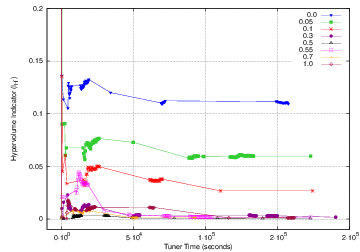
\includegraphics[width=0.45\textwidth]{zeno3e_Add_trajeth.png}}
  \subfloat[ParamILS$_{Fitness}$ on $zeno3_{cost}$]{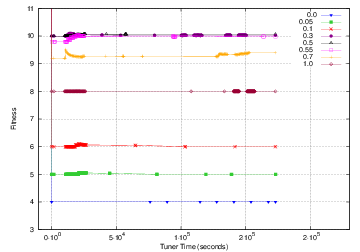
\includegraphics[width=0.45\textwidth]{zeno3e_Add_trajetb.png}}\qquad
  \subfloat[ParamILS$_{H}$ on $zeno3_{risk}$]{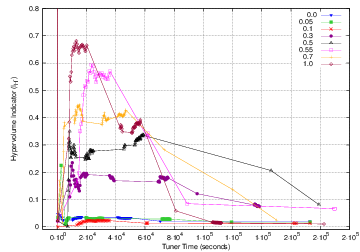
\includegraphics[width=0.45\textwidth]{zeno3e_Max_trajeth.png}}
   \subfloat[ParamILS$_{Fitness}$ on $zeno3_{risk}$]{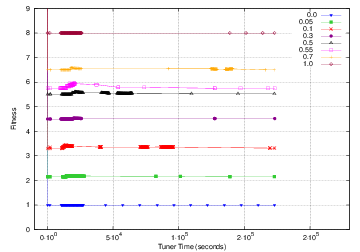
\includegraphics[width=0.45\textwidth]{zeno3e_Max_trajetb.png}}\qquad
  \subfloat[ParamILS$_{H}$ on $zeno6_{cost}$]{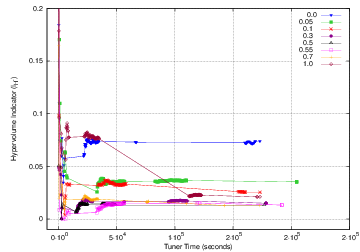
\includegraphics[width=0.45\textwidth]{zeno6e_Add_trajeth.png}}
   \subfloat[ParamILS$_{Fitness}$ on $zeno6_{cost}$]{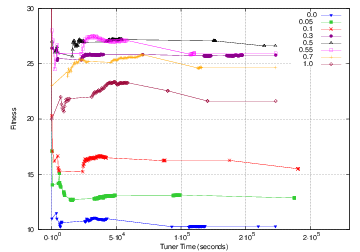
\includegraphics[width=0.45\textwidth]{zeno6e_Add_trajetb.png}}\qquad
 \caption{Sample ParamILS trajectories on MultiZeno instances }
\label{fig:trajectoryParamILS-aggreg1}
 \end{figure}
 
 \clearpage 
\newpage

 \begin{figure}[h!]
\centering  
  \subfloat[ParamILS$_{H}$ on $zeno6_{risk}$]{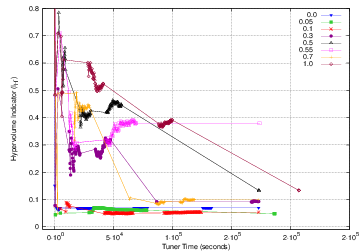
\includegraphics[width=0.45\textwidth]{zeno6e_Max_trajeth.png}} 
  \subfloat[ParamILS$_{Fitness}$ on $zeno6_{risk}$]{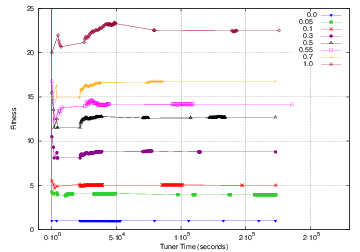
\includegraphics[width=0.45\textwidth]{zeno6e_Max_trajetb.png}}\qquad
  \subfloat[ParamILS$_{H}$ on $zeno9_{cost}$]{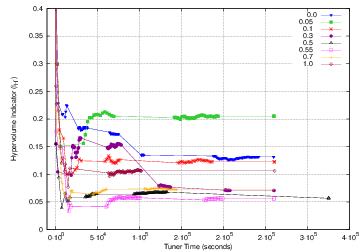
\includegraphics[width=0.45\textwidth]{zeno9e_Add_trajeth.png}}
   \subfloat[ParamILS$_{F}$ on $zeno9_{cost}$]{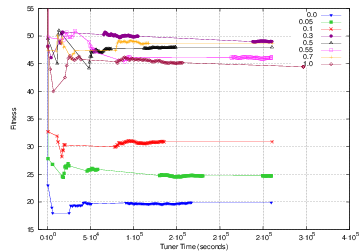
\includegraphics[width=0.45\textwidth]{zeno9e_Add_trajetb.png}}\qquad
   \subfloat[ParamILS$_{H}$on$zeno9_{risk}$]{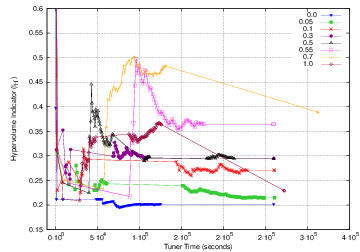
\includegraphics[width=0.45\textwidth]{zeno9e_Max_trajeth.png}}
  \subfloat[ParamILS$_{F}$ on $zeno9_{risk}$]{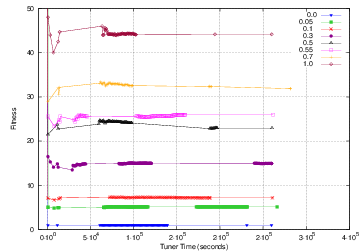
\includegraphics[width=0.45\textwidth]{zeno9e_Max_trajetb.png}}\qquad
 \caption{Sample ParamILS trajectories on MultiZeno instances }
\label{fig:trajectoryParamILS-aggreg2}
\end{figure}


\newpage
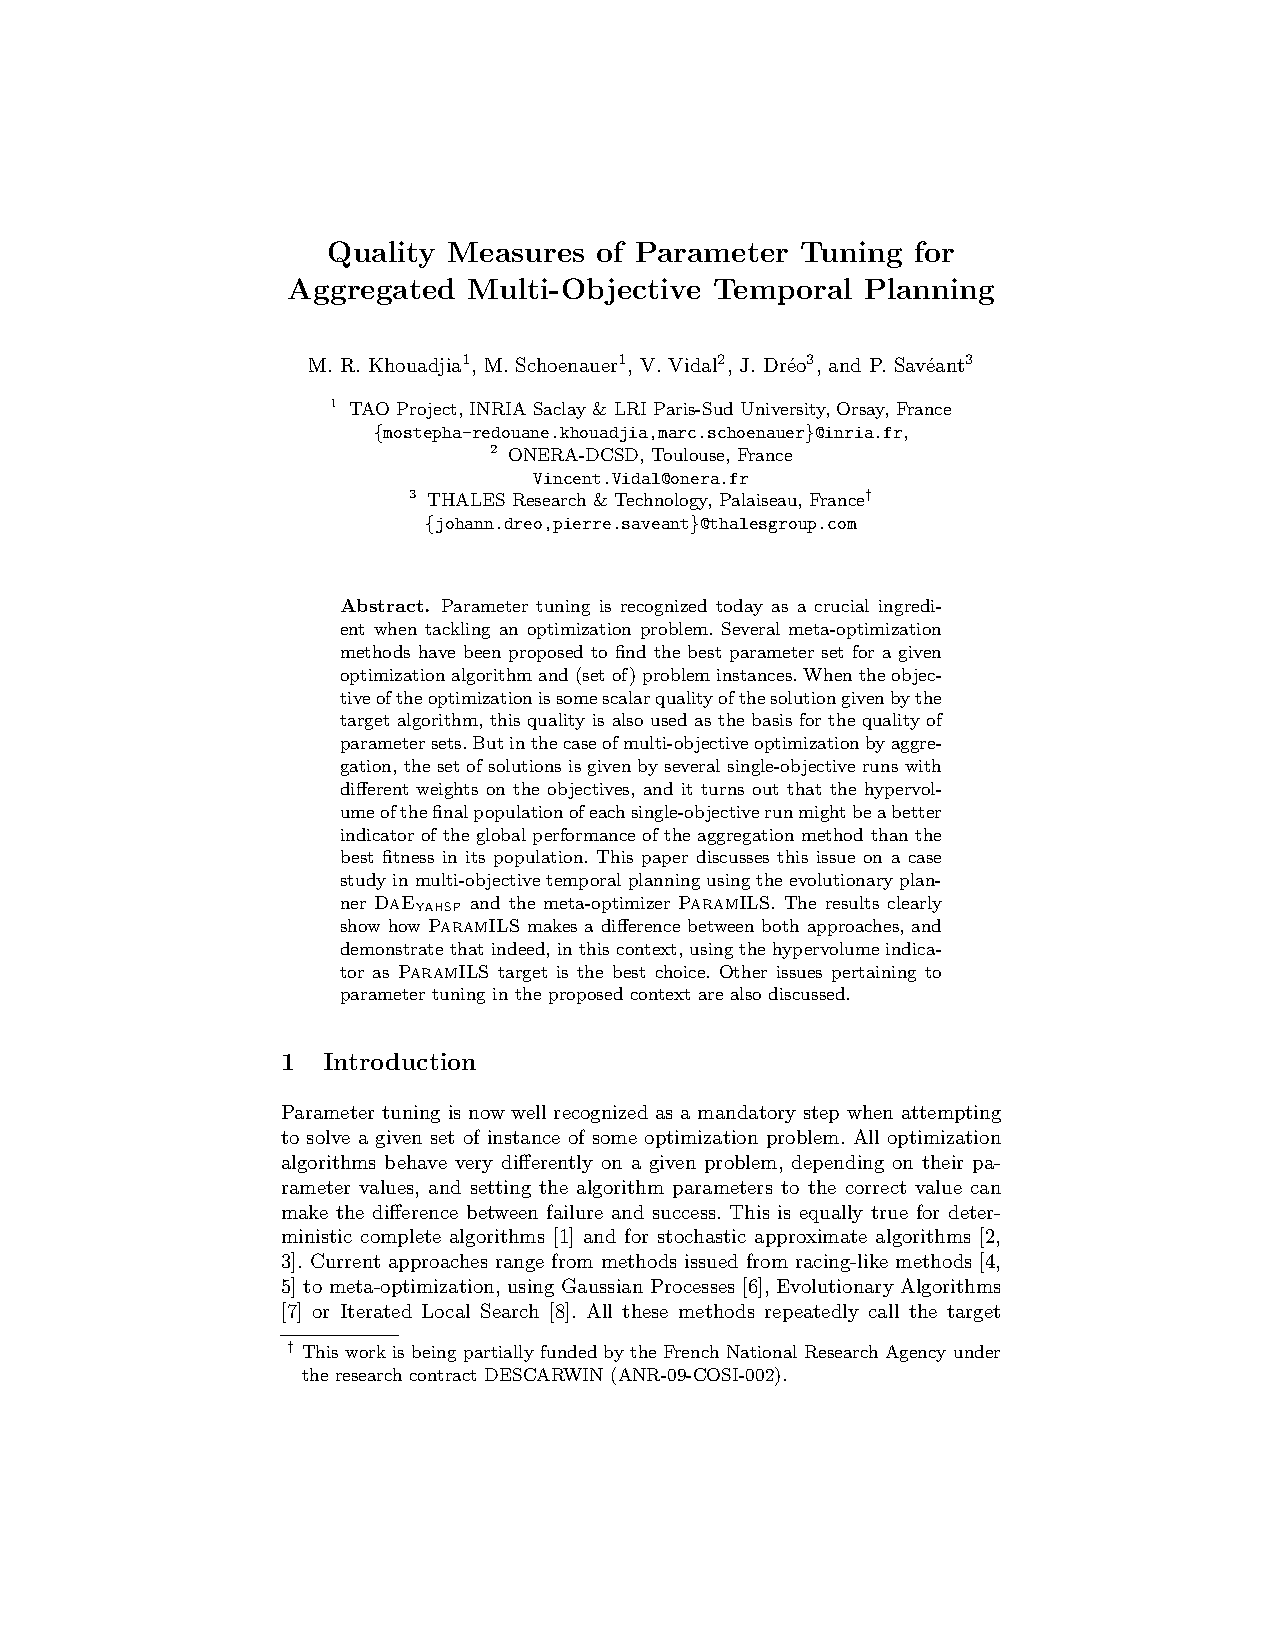
\includepdf[height=32cm,pages=-,offset=2.2cm -4cm]{lion_final.pdf}
\newpage

\chapter{Conclusion}
\label{conclusion}
This Deliverable was supposed to describe works (and results!) about on-line tuning of parameters. Unfortunately, the ideas we had, and the hints we followed, inspired by previous works on the INRIA partner, turned out to be some sort of dead-ends. First, the Adaptive Operator Selection was demonstrated to be useless when facing fitness landscapes with large plateaux (i.e. very few changes in the fitness) when getting close to good individuals. But also, the \LAO\ approach, developed within the project, and which is as close from on-line tuning as you can get when staying at the instance level, also showed some weaknesses, probably suffering from the lack of good features to represent the instance characteristics (something which is not new either, in the Machine Learning community at least).

But the failure of dynamic procedures for on-line parameter tuning is not quite new either in the Evolutionary Computation world: Indeed, as pointed out by Ken DeJong, {\em Perhaps the most interesting thing to note today, after more than 30 years of experimenting with dynamic parameter setting strategies, is that, with one exception, none of them are used routinely in every day practice. The one exception are the strategies used by the Evolution Strategies community for mutation step size adaptation."} (in ``Parameter Setting in EAs: a 30 Year Perspective'', in Lobo, F., Lima, C., Michalewicz, Z., eds., {\em Parameter Setting in Evolutionary Algorithms}, Springer Verlag, 2007).

So it seems that AI Planning will not, at the moment at least, and contrary to what we thought possible when starting the DESCARWIN project, be a second exception to be opposed to Ken Dejong's rather pessimistic statement \ldots

However, the end of this Deliverable (Chapter 5) and the surprising result about ParamILS metric for aggregated approach to multi-objective optimization should convince us that there is always some more work to do, even though sometimes where we were not expecting it -- this is the beauty of scientific research.

% \chapter{References}
% \bibliographystyle{alpha}
% \bibliography{xxx}

\end{document}

%%%%%%%%%%%%%%%%%%%%%%%%%%%%%%%%%%%%%%%%%%%%%
Rapport de r�sultats de Matthias en vue IPC 2011 ?????

Section \ref{section:competition} describes the special settings of our system used in the competition. Finally, Section \ref{section:future} gives some pointers to future plans and work.  


\section{The IPC Competition}
\label{section:competition}

In the Planning and Learning Part of IPC2011 (IPC), there were 5 domains published, with a corresponding problem-generator for each domain. The 5 domains are Ferry, Freecell, Grid, Mprime, and Sokoban. We generated approximately 100 instances for each domain, since this seemed to be appropriate for a running time of 2-3 weeks. The description of the track fixes running time as 15 minutes. Since we use number of evaluations as a terminating criterion, we carried out a run for each instances on our own server to measure the median of number of evaluations for each instance with our default parameters. The median of 11 runs were taken and used as a termination criterion for each instance in the train set. For many instances we did not have any result in 15 minutes, those we had to drop. The remaining instances were used for training. 

 \begin{table*}[ht]
\centering
\begin{tabular}{l c c c c c c}
\hline\hline
Name & \# of iterations & \# of training instances &  ANN-error & quality-ratio \LAO& quality-ratio ANN \\ 
\hline
Ferry & 12 & 32 & 0.17 & 1.06 & 0.59   \\
Freecell& 12 & 108 & 0.08 & 1.09 & 1.05   \\
Grid & 9 & 55 & 0.09 & 1.09 & 1.0   \\
Mprime & 8 & 64 & 0.16 & 1.11 & 1.01 \\
Sokoban & 8 & 32 & 0.11 & 1.22 & 0.79  \\
\hline
\end{tabular}
\label{table:domains}
\caption{Domains: note that only the actually usable training instances are shown. ANN-error is given as MSE, returned by FANN}
\end{table*} 

\begin{table*}[ht]
\centering
\begin{tabular}{l c c c}
\hline\hline
Name & Minimum & Maximum & Default value \\ 
\hline
Probability of crossover & 0.0 & 1 & 0.8 \\
Probability of mutation & 0.0& 1& 0.2 \\
Rate of mutation add station& 0& 10& 1 \\
Rate of mutation delete station& 0& 10& 3 \\
Rate of mutation add atom& 0& 10& 1 \\
Rate of mutation delete atom& 0& 10& 1 \\
Mean average for mutations& 0.0& 1& 0.8 \\
Time interval radius& 0& 10& 2 \\
Maximum number of stations& 5& 50& 20 \\
Maximum number of nodes& 100& 100000& 10000 \\
Population size& 10& 300& 100 \\
Number of offsprings& 100& 2000& 700 \\
\hline
\end{tabular}
\label{table:parameters}
\caption{Controlled Parameters}
\end{table*} 

Table \ref{table:domains} shows the data for each domain, as you can see from the approximately 100 instances from each domain we could only use all instances in the domain Freecell. In the other domains we got much less usable instances. The Mean Square Error (MSE) is shown for each domain. Note that since there can be multiple optimal parameters for the same instance (fitness-function is discrete), there might be an unavoidable error of the ANN.

5 iterations of CMA-ES were carried out, followed by one ANN and one gene-transfer, and this cycle were iterated in the algorithm. This means that for example CMA-ES was running for 50 iterations for the Grid domain.

The ANN had 3 fully connected layers, and the hidden layer had the same number of neurons as the input. Learning was done by the conventional back-propagation algorithm, which is the default in FANN. The ANN was only trained for 50 iterations in one iterations of \LAO, so that we avoid over-training. Over the 10 iterations of \LAO\ this means that 500 iterations of the ANN was carried out.

Termination criterion in the competition was simply the available time, the algorithm was running for several weeks parallel on our cluster, which is used also for other research, i.e. only a small number of 4 or 8-core processors were available for each domain in average.

The parameters of DAEx controlled are described in table \ref{table:parameters}. For a detailed description of these parameters, see \cite{BibGECCO:2010}. The feature set consists of the number of fluent, goals predicates objects and types in the domain or instance, respectively. One further feature is called mutex density, which is the number of mutexes divided by the number of all fluent-pairs. We also added number of lines, words and byte-count - obtained by the linux command called "wc" - of the instance and the domain file as some not so serious, primitive features.

\section{Future Work}
\label{section:future}	

Since \LAO\ is only a framework, as indicated other kind of learning methods, and other kind of optimization techniques may be tried. Also the benefit of gene-transfer and/or cross-over might be investigated further. One shall also test, how inter-domain generalization works. Maybe it is possible to learn a mapping for all the domains, since the features may grasp the specificity of a domain. Naturally, the set of features may always be extended, or tested. Feature-selection would become important only if data with a considerable number of features and instances are present. This is not the case yet.
